\documentclass[10pt,twocolumn,letterpaper]{article}

%\usepackage[showframe]{geometry}
\usepackage{geometry}
\usepackage{cvpr}
\usepackage{times}
\usepackage{epsfig}
\usepackage{graphicx}
\usepackage{amsmath}
\usepackage{amssymb}
\usepackage{soul}
\usepackage[]{mcode}
\usepackage{caption} 
\captionsetup[table]{skip=10pt}

\setlength{\voffset}{-50pt}
%\setlength{\hoffset}{-25pt}
%!TEX encoding = UTF-8 Unicode\setlength{\headsep}{2pt}
\setlength{\textheight}{715pt}
%\setlength{\textwidth}{511pt}

% Include other packages here, before hyperref.

% If you comment hyperref and then uncomment it, you should delete
% egpaper.aux before re-running latex.  (Or just hit 'q' on the first latex
% run, let it finish, and you should be clear).
\usepackage[breaklinks=true,bookmarks=false]{hyperref}

\cvprfinalcopy % *** Uncomment this line for the final submission

\def\cvprPaperID{****} % *** Enter the CVPR Paper ID here
\def\httilde{\mbox{\tt\raisebox{-.5ex}{\symbol{126}}}}

% Pages are numbered in submission mode, and unnumbered in camera-ready
%\ifcvprfinal\pagestyle{empty}\fi
% \setcounter{page}{1}
\begin{document}

%%%%%%%%% TITLE
\title{Deep Learning Project: Using Bayesian Optimization to Find Good Augmentation Policies from Data}

\author{
    	\small{NAMES: Samuel Frommenwiler, Gian K\"onig} \\
   	\small{NETHZ: fsamuel, koenigg}\\
	\small{EMAIL: \{fsamuel, koenigg\}$@$student.ethz.ch}\\
    	\small{ID: 08-738-601, 09-913-245}
}

\maketitle
%\thispagestyle{empty}

%%%%%%%%% ABSTRACT
\begin{abstract}
This document presents the results for the deep learning course at ETH as required in~\cite{DL18}. In the first section data augmentation as the problem of interest is described, as well as reinforcement learning as an approache to improve data augmentation. In the second section, the problem is described in more detail and Bayesian Optimization is introduced as an alternative approach to tune hyper parameters for automated data-augmentation policies. This section also includes the final results. Finally, a conclusion is presented. 
\end{abstract}

%%%%%%%%% BODY TEXT
\section{AutoAugment with Reinforcement Learning and Other Approaches}
Machine learning algorithms usually achieve better results with more data, however acquiring this additional data can be expensive and time-consuming.  A common trick to increase the amount of training data is to add copies of existing data with small perturbations to the training set. For a dataset of natural images dataset augmentation methods include random cropping, image mirroring, rotation, color shifting and color whitening. Picking a good combination of these methods is usually done by hand and requires expert knowledge and time.
\par
Therefore, an automated approach was introduced in order to find the best policies~\cite{Ekin}. Cubuk et. al. present a process of finding an efficient data augmentation policy, in which each policy contains possible augmentation operations. Each operation contains an image processing function (e. g. translation, rotation or color normalization) combined with a probability that this function is applied with a corresponding magnitude. To find the best choices of these functions and suitable scaling factors, Cubuk et. al. use a reinforcement learning search algorithm such that a neural network, trained on these hyper parameters, yields the best validation accuracy. 
\par
Geng et al. \cite{DBLP:journals/corr/abs-1811-04768} extended on this idea using augmented random search to efficiently find augmentation policies in a continuous hyper parameter search space. Tran et al. \cite{DBLP:journals/corr/abs-1710-10564} follow a slightly different approach where they use GANs to find valid augmented data. While Fawzi et al. \cite{Fawzi} pursued a worst-case augmentation approach where they generate augmented data which gives the biggest loss for the current classifier.

\section{AutoAugment with Bayesian Optimization}
We use Bayesian Optimization, a technique already used for tuning hyperparameters, to automatically select a good combination of augmentation policies. And to compare this to the approach used in~\cite{Ekin}. Specifically, we investigate the Bayesian Optimization \cite{2018arXiv180702811F},~\cite{Goodfellow-et-al-2016} approach with a Tree Parzen Esimator~\cite{Kaggle_AMT} by using the Hyperopt library~\cite{HyperOpt} with the help of~\cite{BO_Hyperopt}. For this specific task,~\cite{2017arXiv171010564T} gives us a guideline on how to integrate Bayesian Optimization into the data augmentation task.
\par
We will focus on using a single network architecture (WideResNet), using the same hyper parameters as the authors of the original paper~\cite{Ekin}, changing the search space from discrete to continuous and utilizing Bayesian Optimization to select the optimal combination of augmentation policies. 

\subsection{Available Policies}
The available policies~\cite{Ekin} used in their program are ShearX(Y) (shear the image along the horizontal (vertical) axis with rate magnitude), TranslateX(Y) (translate the image in the horizontal (vertical) direction by magnitude number of pixels), Rotate (rotate the image magnitude degrees), AutoContrast (maximize the the image contrast, by making the darkest pixel black and lightest pixel white),  Invert (invert the pixels of the image), Equalize (equalize the image histogram), Solarize (invert all pixels above a threshold value of magnitude), Posterize (reduce the number of bits for each pixel to magnitude bits), Contrast (control the contrast of the image. A magnitude=0 gives a gray image, whereas magnitude=1 gives the original image), Color (adjust the color balance of the image, in a manner similar to the controls on a colour TV set. A magnitude=0 gives a black and white image, whereas magnitude=1 gives the original image), Brightness (adjust the brightness of the image. A magnitude=0 gives a black image, whereas magnitude=1 gives the original image), Sharpness (adjust the sharpness of the image. A magnitude=0 gives a blurred image, whereas magnitude=1 gives the original image), Cutout (set a random square patch of side-length magnitude pixels to gray), Sample Pairing (linearly add the image with another image (selected at random from the same mini-batch) with weight magnitude, without changing the label).
The code which includes the reinforcement learning to generate the optimal policies is not included in their repository\footnote{https://github.com/tensorflow/models/tree/master/research/autoaugment}. But the results from the optimization is included in the file \texttt{policies.py}, or in table 8 in~\cite{Ekin}. Figure~\ref{fig:PolicyExample} shows samples of the policies applied to some images from the CIFAR-10.

\begin{figure}
	\centering
	\resizebox{\columnwidth}{!}{
	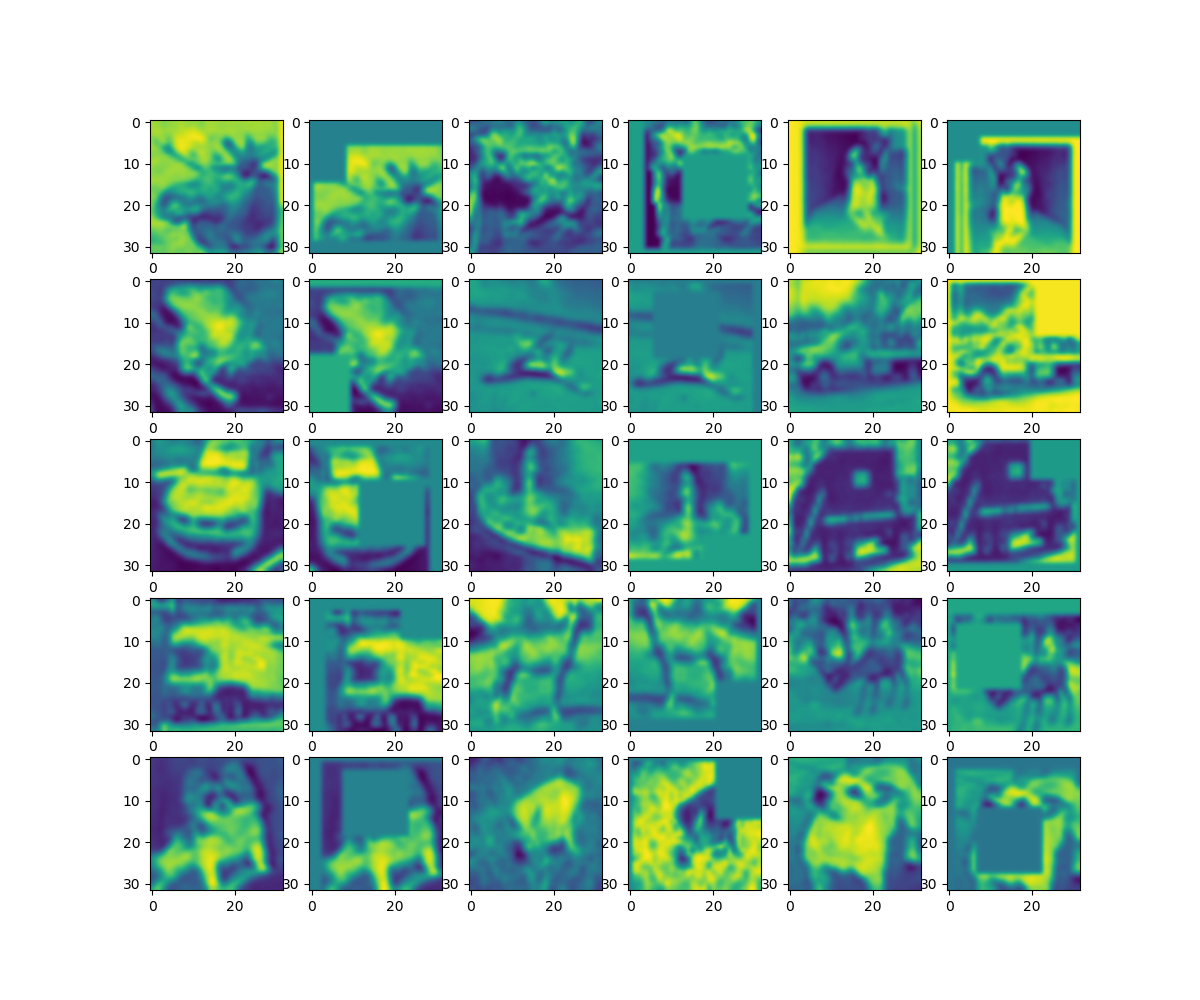
\includegraphics{../autoaugment/policy_examples_20181228-165922.png}
	}
	\caption{Example of policies found with RF applied to CIFAR-10}
	\label{fig:PolicyExample}
\end{figure}

\subsection{Generate Optimal Policies using Bayesian Optimization}
Because our computation power was limited, we decided to use only the 25 sub-policies listed in table~\ref{tab:good_policies} found by~\cite{Ekin} and optimize over the probability and magnitude of each of the sub-policy.

The following procedure briefly describes the steps of the process to find optimal probability and magnitude for each sub-policy defined in~\ref{tab:good_policies} with reference to the files in our repository\footnote{https://github.com/giankoenig/DL18}:

\begin{enumerate}
\item Run \texttt{DL18/dl\_mix/eval\_policies.py} $\rightarrow$ A WRN-40-2 is trained on a reduced CIFAR-10 data set for each sub-policy defined in the \texttt{DL18/dl\_mix/search\_space.py}. The optimal policies are safed in the folder \texttt{DL18/trials}.
\item Run \texttt{DL18/read\_trials.py} $\rightarrow$ This creates the file \texttt{optimal\_policies\_[X].pol}, which includes the optimal policies in a structure that can be processed by the main program \texttt{train\_cifar.py}. In order to read in the new good policies, the file \texttt{hyperopt\_policies.py} is placed \texttt{DL18/autoaugment} and called on \texttt{line 51} in \texttt{data\_utils.py} in order to import the new policies.
\item Run \texttt{DL18/autoaugment/train\_cifar.py} $\rightarrow$  Trains CIFAR-10 on WRN-28-10 with optimal policies.
\end{enumerate}

To run the training in step 1 and 3 above it is suggested to use \texttt{nohup [COMMAND] $>$ output.txt $\&$} in order to store the output of the program. Note: To abort a command start with that setting, first find the ID of the job with \texttt{ps aux | grep python} and then abort it with \texttt{kill [JOB\_NUMBER]}. Below \texttt{[COMMAND]} for step 3 is given:

\begin{table}[h!]
\begin{center}
\begin{tabular}{lllll}
 &\texttt{python train\_cifar.py}  \\
 &\qquad \qquad \texttt{--model\_name=wrn}  \\
 &\qquad \qquad \texttt{--checkpoint\_dir=../training/}   \\
 &\qquad \qquad \texttt{--data\_path=../../data/}  \\
 &\qquad \qquad \texttt{--dataset='cifar10'} \\
 &\qquad \qquad \texttt{--use\_cpu=0}
\end{tabular}
\end{center}
\end{table}

\subsection{Results}
We performed three trainings where we optimized the probabilities and magnitude of the good policies~\ref{tab:good_policies}. A first run with 10 trials for each policy and 10 epochs on the WRN-40-2, a second one with 20 additional trials for each policy and again 10 epochs. For the last run the search space was slightly adjusted because some found policies from the second round seemed unreasonable. In order to increase accuracy the number of trials was increased to 20 per policy and the epoch number was increased to 12. The results are listed in the table~\ref{tab:results} below.
\begin{table}[h!]
\begin{center}
\begin{tabular}{lllll}
\hline
& Train Acc: &Test Acc: \\
\hline
Reinforcement Learning & None & 0.9727 \\
Bayesian Optimization$_{S1,10,10}$ & 0.9353 & 0.9728 \\
Bayesian Optimization$_{S1,10,30}$ & 0.9354 & 0.9684 \\
Bayesian Optimization$_{S2,12,20}$ & tbd & tbd \\
\hline
\end{tabular}
\caption {Simulation results} \label{tab:results} 
\end{center}
\end{table}

We performed the training on the Google Cloud~\cite{GCloud} using one Tesla P100 GPU. The training of the WRN-28-10 with the policies given from the reinforcement learning search required 9h15min. The time required to optimize all probabilities and magnitudes of the policies~\ref{tab:good_policies} with 20 trials for each subpolicy required 12.5h. \newline



\section{Appendix}

\subsection{Other Infrastructure}
A first attempt to run the code on the CPU with MacBook Pro (Retina, 15-inch, Early 2013) with 2.4 GHz Intel Core i7, 16 GB 1600 MHz DDR3, Intel HD Graphics 4000 1536 MB, macOS Sierra 10.12.5 resulted in a Training Time: of \texttt{INFO:tensorflow:Epoch time(min): 332.056} \newline

We tried to execute the code on the Leonhard Cluster\footnote{https://scicomp.ethz.ch/wiki/Leonhard}. For this the following commands were necessary. 1) \texttt{ssh [NETHZ]@login.leonhard.ethz.ch} 2) Create folders and git clone or upload the data from PC \texttt{rsync -Pav ~/PATH [NETHZ]@login.leonhard.ethz.ch:/[PATH])} and 3) Load the right moduel with \texttt{module load python\_gpu/2.7.13} (module list: Currently Loaded Modules: 1) StdEnv   2) gcc/4.8.5   3) openblas/0.2.19   4) cuda/8.0.61   5) cudnn/6.0   6) jpeg/9b   7) libpng/1.6.27   8) python\_gpu/2.7.13) 4) Execute the code: \texttt{bsub -n 20 -R "rusage[mem=4500,ngpus\_excl\_p=1]" python train\_cifar.py --model\_name=wrn --checkpoint\_dir=tmp/training/ --data\_path=tmp/data/ --dataset='cifar10' --use\_cpu=0}. \newline

It turns out on the Leonhard Cluster we can only use 1 GPU and also each job has a time limit of 4h. For this run, we could analyze the output using \texttt{grep -A3 "Creating TensorFlow device" lsf.o1058716} which shows that in 4 hours only 47 epochs were executed. From the data below we can see that one epoch uses approximately 5 minutes. Another problem was that when we wanted to start a job, the waiting for a very long time (up to 24h). \newline

\noindent
[koenigg@lo-login-02 model]\$ ls -l
total 570652
-rw-rw---- 1 koenigg koenigg-group       127 Jan  8 13:49 checkpoint
-rw-rw---- 1 koenigg koenigg-group 289836892 Jan  8 \textbf{13:44} model.ckpt-40.data-00000-of-00001
-rw-rw---- 1 koenigg koenigg-group      9868 Jan  8 13:44 model.ckpt-40.index
-rw-rw---- 1 koenigg koenigg-group   1163579 Jan  8 13:44 model.ckpt-40.meta
-rw-rw---- 1 koenigg koenigg-group 289836892 Jan  8 \textbf{13:49} model.ckpt-41.data-00000-of-00001
-rw-rw---- 1 koenigg koenigg-group      9868 Jan  8 13:49 model.ckpt-41.index
-rw-rw---- 1 koenigg koenigg-group   1163579 Jan  8 13:49 model.ckpt-41.meta \newline

\noindent
[koenigg@lo-login-01 model]\$ date
Thu \textbf{Jan 10 09:45:45} CET 2019
[koenigg@lo-login-01 model]\$ bjobs
JOBID USER STAT QUEUE FROM\_HOST EXEC\_HOST JOB\_NAME SUBMIT\_TIME 1060305 koenigg PEND gpu.4h lo-login-01 *use\_cpu=0 \textbf{Jan  9 22:00}\newline

Therefore using Leonhard was not a practical solution to train the models.\newline

\noindent
\textbf{Note}: Useful commands: \texttt{bjobs} to show the jobs (with option -l for more details), \texttt{module avail} to show available modules, \texttt{module list} to show loaded modules, \texttt{ls -l --block-size=M} to show detailed files with size in MB, Sync simulation results to local computer: rsync -chavzP --stats koenigg@login.leonhard.ethz.ch:/.../model.ckpt-199.meta $\sim$/.../autoaugment/tmp/training/model/. \newline

\begin{table}[h]
\begin{center}
\begin{tabular}{lll}
\hline
& Operation 1 & Operation 2 \\
\hline
Sub-policy 0 & Invert & Contrast \\
Sub-policy 1 & Rotate & TranslateX \\
Sub-policy 2 & Sharpness & Sharpness \\
Sub-policy 3 & ShearY & TranslateY \\
Sub-policy 4 & AutoContrast & Equalize \\
Sub-policy 5 & ShearY & Posterize \\
Sub-policy 6 & Color & Brightness \\
Sub-policy 7 & Sharpness & Brightness \\
Sub-policy 8 & Equalize & Equalize \\
Sub-policy 9 & Contrast & Sharpness \\
Sub-policy 10 & Color & TranslateX \\
Sub-policy 11 & Equalize & AutoContrast \\
Sub-policy 12 & TranslateY & Sharpness \\
Sub-policy 13 & Brightness & Color \\
Sub-policy 14 & Solarize & Invert \\
Sub-policy 15 & Equalize & AutoContrast \\
Sub-policy 16 & Equalize & (Equalize \\
Sub-policy 17 & Color & Equalize \\
Sub-policy 18 & AutoContrast & Solarize \\
Sub-policy 19 & Brightness & Color \\
Sub-policy 20 & Solarize & AutoContrast \\
Sub-policy 21 & TranslateY & TranslateY \\
Sub-policy 22 & AutoContrast & Solarize \\
Sub-policy 23 & Equalize & Invert \\
Sub-policy 24 & TranslateY & AutoContrast \\
\hline
\end{tabular}
\caption {Search Space: These policies are used and the probability (P) and magnitude (M) attached to each operation is optimized.} \label{tab:good_policies} 
\end{center}
\end{table}

{\small
\bibliographystyle{ieee}
\bibliography{dlbib}
}

\end{document}
